\subsection{Red Black Gauss-Seidel iterations}

To solve the linear system $A\vec{p} = \vec{b}$ we are going to use an iterative solving method called Red-Black Gauss-Seidel. $A$ is a Laplacian matrix and therefore each linear system has the following form

\begin{equation}
{A}^{center}_{i,j} p_{i,j} + {A}^{left}_{i,j} p_{i-1,j} + {A}^{right}_{i,j} p_{i+1,j} + {A}^{bottom}_{i,j} p_{i,j-1} + {A}^{top}_{i,j} p_{i,j+1} = b_{i,j}
\label{laplaceAeq}
\end{equation}

If we rearrange Equation \ref{laplaceAeq} and use the notion $p^n$ for current pressure value and $p^{n+1}$ for the next updated value we get

\begin{equation}
{p}^{n+1}_{i,j}  = -\frac{ {A}^{left}_{i,j} {p}^{n}_{i-1,j} + {A}^{right}_{i,j} {p}^{n}_{i+1,j} + {A}^{bottom}_{i,j} {p}^{n}_{i,j-1} + {A}^{top}_{i,j} {p}^{n}_{i,j+1}}{{A}^{center}_{i,j}} + b_{i,j}
\label{jacobi}
\end{equation}

If we would iterate over all cells in our grid in each iterations step and use Equation \ref{jacobi}, it would be called Jacobi iterations. Instead, we are going to use a Gauss-Seidel approach that converges faster than Jacobi iterations. The key is in which order we update the pressure. In Red-Black Gauss-Seidel we only update the pressure in a cell every other iteration step. If a cell $(i,j)$ is updated in an iteration step $n$, the neighbords of that cell will not be updated. In iteration step $(n+1)$, the cell $(i,j)$ is not updated but instead all the neighbors are. Figure \ref{redblack} shows how all the cells in a two dimensional grid are being divided to either a red or black set. On even iteration steps, we update the red cells and on uneven steps we update the black cells.

\begin{figure}[ht!]
\centering
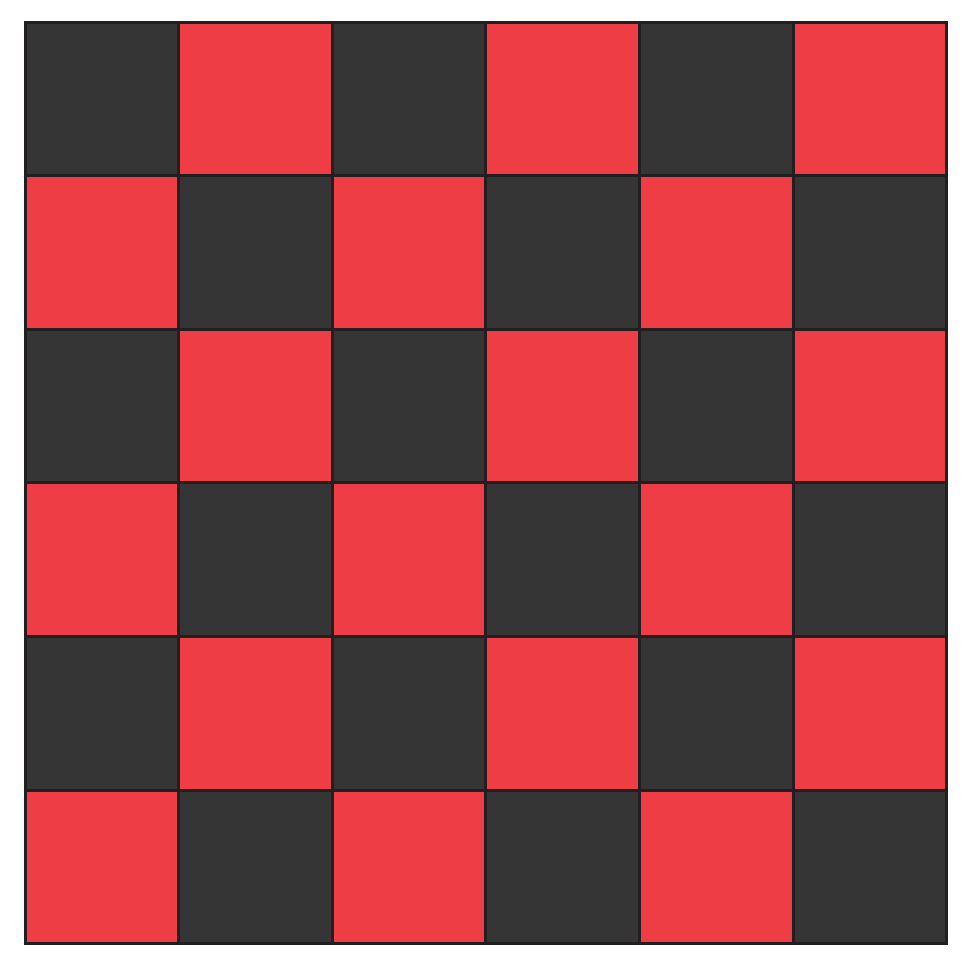
\includegraphics[width=55mm]{img/redblack.pdf}
\caption{In Red Black Gauss-Seidel iterations, the grid domain is divided in to a red and a black region. Only cells within a subregion are updated every other iterations tep..}
\label{redblack}
\end{figure}
